%!TEX root = ../adrien_gomar_phd.tex

\section{Detailed algorithm to compute \texorpdfstring{$\varepsilon_1$}{e1}}
\label{app:epsilon_1_steps}

A sketch of the steps used to 
evaluate $\varepsilon_1$ from a computation is 
shown in Figure~\ref{fig:CRITERION_1}.
Two azimuthal lines are extracted in the
stator and in the rotor respectively (step~\textcircled{\small{1}}). 
These are duplicated using the phase-lag
condition to retrieve the full $2 \pi$ signal in both 
blocks. The
axial momentum $\rho U$ variable is analyzed. The main advantages of
this variable are that it is a representative variable
for the wake, it is a conservative variable of the considered governing 
equations and finally, it is invariant under a change of reference frame, 
unlike the relative velocities for instance.
Then, an azimuthal Fourier transform,
denoted $\mathcal{F}_\theta$, is carried out on each azimuthal $2 \pi$ signals 
and gives the frequency content
of the wake in both the stator and the rotor (step~\textcircled{\small{2}}).
\begin{figure}[htp]
  \centering
  \includegraphics*[width=0.6\textwidth]{CRITERION_1.pdf}
  \caption{Sketch of the steps needed to 
  compute the first error quantification $\varepsilon_1$.}
  \label{fig:CRITERION_1}
\end{figure}
However, due to the time interpolation 
between the two rows achieved 
at the interface, spurious effects can 
appear upstream the interface as shown in Figure~\ref{fig:rb_spurious_interf}. 
The effects of the rotor block are significant on the 
closest cells to the interface for the $N=5$ computation 
and still appear on the very lasts cells before the 
interface for the $N=10$ computation. 
They have disappeared when using $N=15$ harmonics.
To lessen the influence of this interpolation, and thus
the spurious effects,
the extraction of the axial momentum 
is not performed at the closest 
cell to the interface. If $d_{ref}$ is 
the axial length of a block, the extraction is achieved 
at $d_{ref} / 5$ of the interface upstream and downstream
the stator and rotor block, respectively. 
It represents six time the length of a cell 
in the axial direction.
As the governing equations are the Euler ones, 
there is no significant variation of the wake thickness 
within six cells, supporting this approach.
Moreover, preliminary studies have shown that $d_{ref} / 5$ is 
sufficient
to lower the spurious effects while keeping the
results consistent.
\begin{figure}[htp]
\centering
  \subfigure[$N=5$]{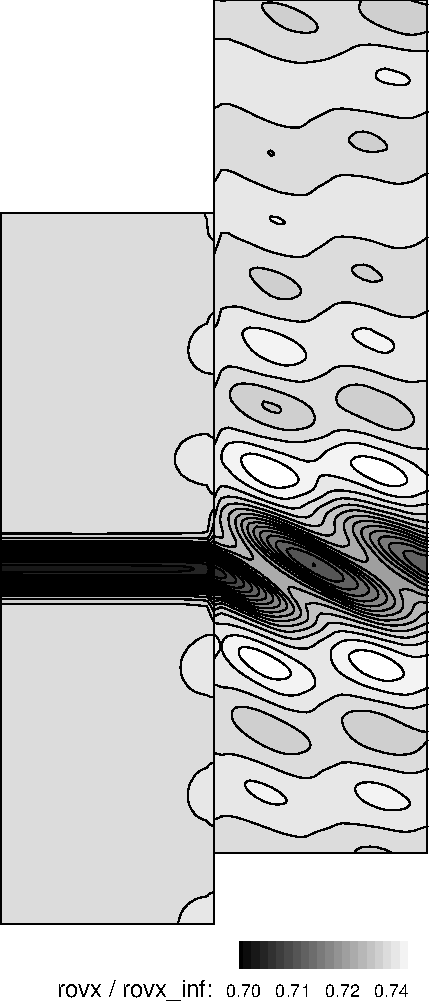
\includegraphics[width=.2\textwidth]{cut_plane_N05_adim.eps}}\quad
  \subfigure[$N=10$]{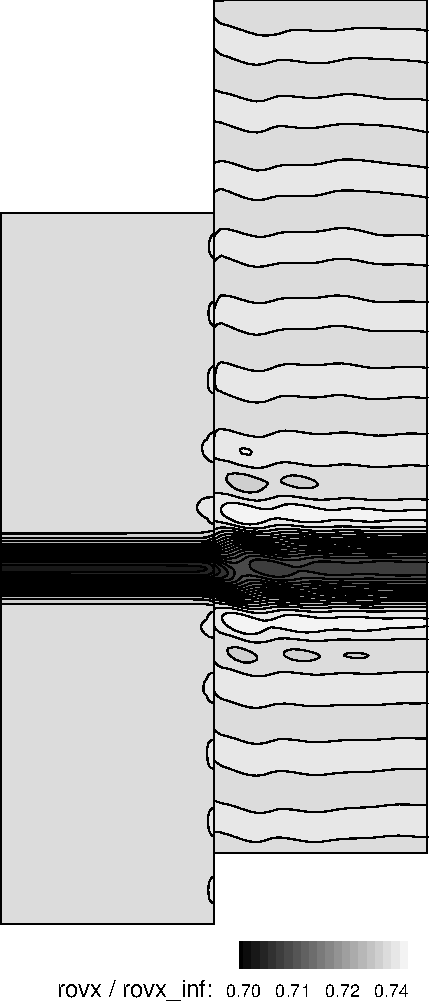
\includegraphics[width=.2\textwidth]{cut_plane_N10_adim.eps}}\quad
  \subfigure[$N=15$]{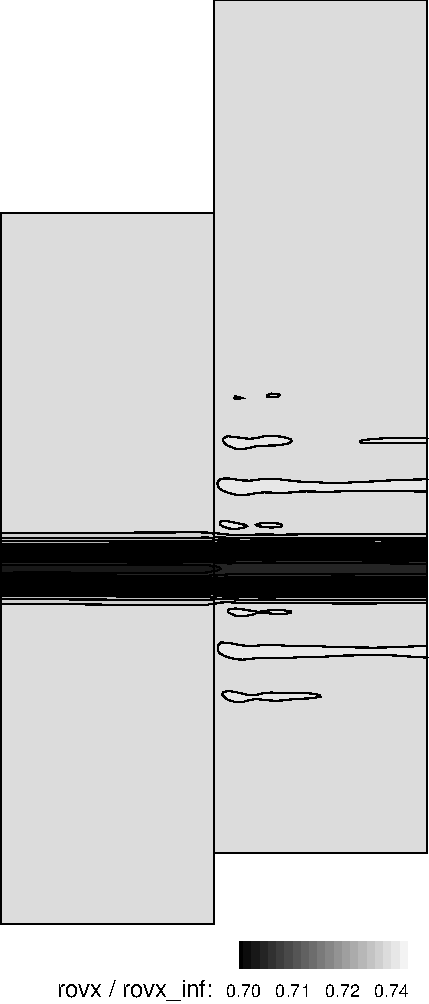
\includegraphics[width=.2\textwidth]{cut_plane_N15_adim.eps}}
  \caption{Occurrence of spurious effects upstream 
  the interface between stator and rotor blocks for a $L=5\%$ wake width.}
  \label{fig:rb_spurious_interf}
\end{figure}

\section{Detailed algorithm to compute \texorpdfstring{$\varepsilon_2$}{e2}}
\label{app:epsilon_2_steps}

The steps to compute
the second error quantification for each 
of the 375~computations, 
are schematically shown
in Figure~\ref{fig:CRITERION_2}. An azimuthal line is extracted
in the stator domain,
nearby the interface (step~\textcircled{\small{1}}), like
for the first error quantification. 
Contrary to this last, in the rotor
block, a time probing is done at one point 
giving an unsteady time
signal of $\rho U(t)$ (step~\textcircled{\small{1}}\textsuperscript{$\prime$}). 
The azimuthal signal is
duplicated using the phase-lag condition 
to retrieve the full $2 \pi$ signal. 
The temporal and spatial signals are then
Fourier transformed so that their spectrum can be compared (step~\textcircled{\small{2}}).
\begin{figure}[htp]
  \centering
  \includegraphics*[width=0.6\textwidth]{CRITERION_2.pdf}
  \caption{Sketch of the steps needed to compute 
  the second error quantification.}
  \label{fig:CRITERION_2}
\end{figure}
The wake extraction is performed at the same axial 
distance of the interface as 
for the first error quantification.
In this case, the location 
of the point in the rotor block has a direct impact on 
the results especially when the wake is under-resolved.
To highlight this impact, the temporal Fourier transform is 
evaluated at two different locations called loc~1 and 
loc~2. The two points are separated 
by a distance $\Delta \theta_{loc_1-loc_2} = d_{ref} / 10$ in the azimuthal direction, 
as shown in Figure~\ref{fig:CRITERION_2}.

\section{Detailed algorithm to the tangential accumulated energy from a mixing plane computation}
\label{app:epsilon_cror_steps}
Figure~\ref{fig:criterion_cror} shows the different steps: firstly, the row
interface is extracted from a mixing-plane computation.
Secondly, using this interface,
the axial momentum is extracted for several spanwise positions in the region of interest
(step~\textcircled{\small{1}}).
In a CROR configuration this is the region with a 
relative span ranging between 0\% and 120\%.
In fact, beyond the 120\% threshold, the influence of the blades on fluid
unsteadiness decreases rapidly such that the fluid 
has a narrow spectrum as the whole spectrum energy lies in, at
most, the first three harmonics.
Then, for each radius, an azimuthal Fourier transform
is performed to obtain the tangential spectrum of the
axial momentum (step~\textcircled{\small{2}}).
\begin{figure}[htp]
  \centering
  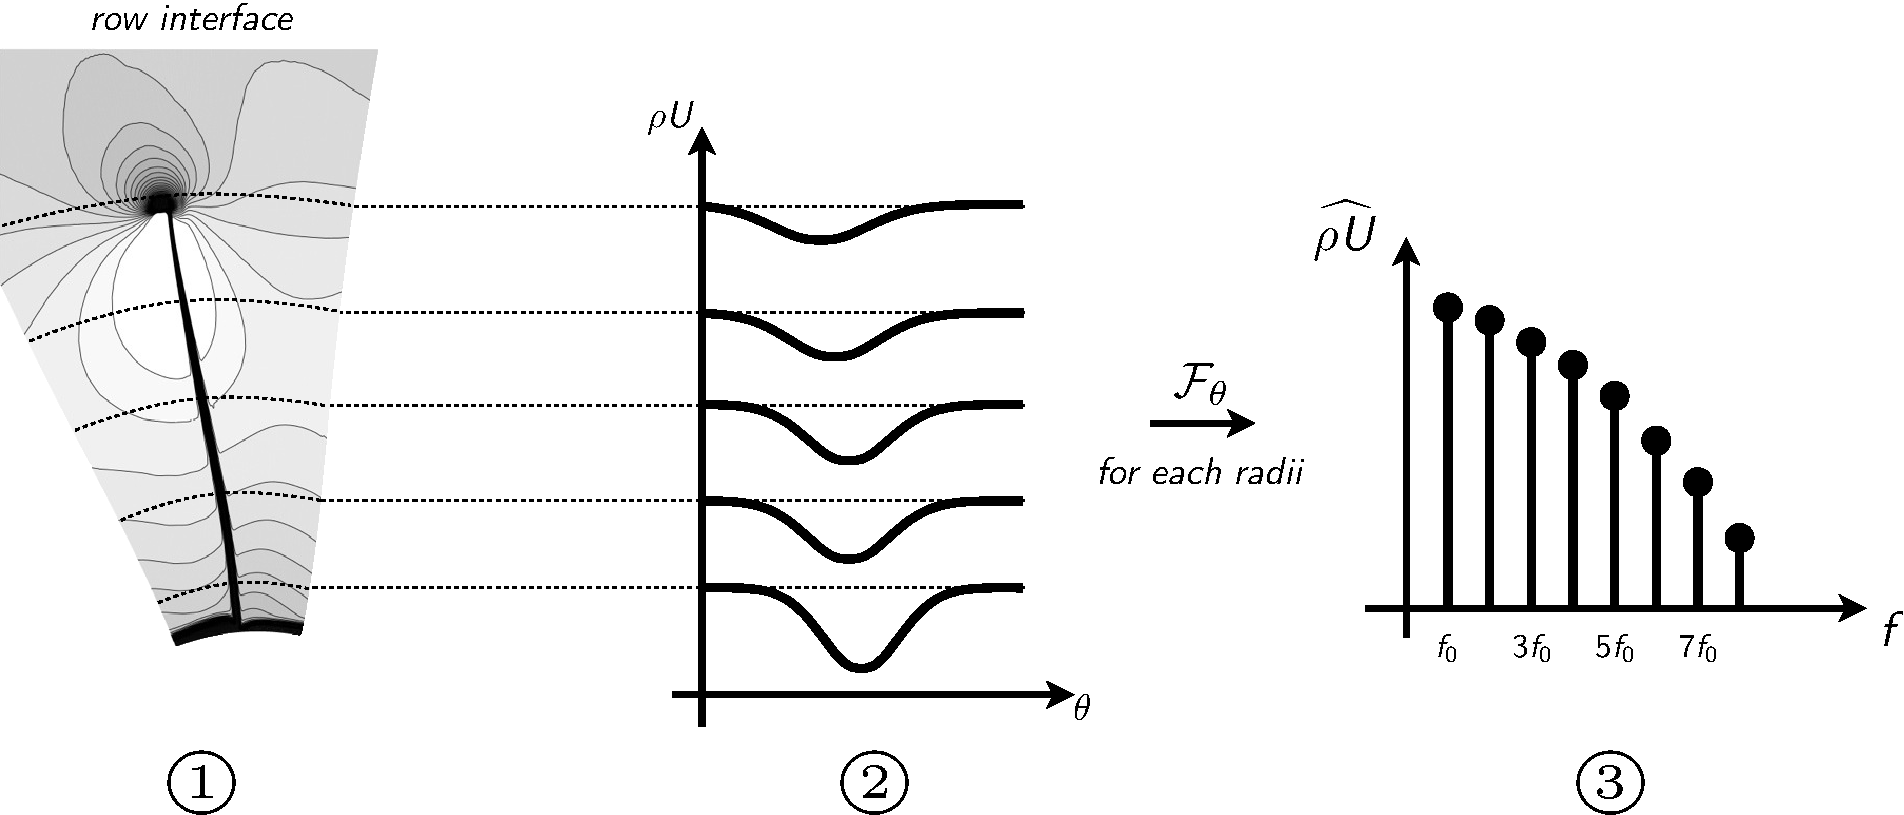
\includegraphics[width=.6\textwidth]{CRITERION_CROR.pdf}
  \caption{Steps for the prediction tool based on an azimuthal
  Fourier transform of the axial momentum at the rotor-rotor interface.}
  \label{fig:criterion_cror}
\end{figure}
The relative cumulative energy for a given number of harmonic $N$ is then defined as:
\begin{equation}
    E (N) = \frac{\sum_{k=1}^N \left[ \widehat{\rho U}^{\theta} (k) \right]^2}{ 
    \sum_{k=1}^\infty \left[ \widehat{\rho U}^{\theta} (k) \right]^2},
    \label{eq:def_crit_cror}
\end{equation} 
where $\widehat{\rho U}^{\theta}$ denotes the axial momentum spectrum
extracted from the rows interface plane. In Eq.~\eqref{eq:def_crit_cror},
the cumulative energy up to harmonic $N$ is 
compared to the total energy.
